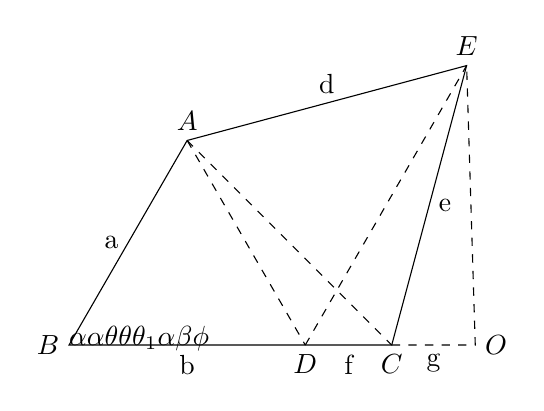
\begin{tikzpicture}
%Marking coordiantes

\coordinate [label=above:$A$] (A) at (1.5,2.59807621);
\coordinate [label=left:$B$] (B) at (0,0);
\coordinate [label=below:$C$] (C) at (4.09807621,0);
\coordinate [label=below:$D$] (D) at (3,0);
\coordinate [label=above:$E$] (E) at (5.04903811,3.54903811);
\coordinate [label=right:$O$] (O) at (5.15873638,0);

%Drawing quadrilaterl ABCE
\draw (A) -- node[left] {$\textrm{a}$} (B) -- node[below] {$\textrm{b}$} (D) -- node[below] {$\textrm{f}$} (C) -- node[right] {$\textrm{e}$} (E) -- node[above] {$\textrm{d}$} (A);
\draw[dashed] (D) -- (E);
\draw[dashed] (A) -- (D);
\draw[dashed] (C) -- node[below] {$\textrm{g}$} (O) -- (E);
\draw[dashed] (A) -- (C);

%Drawing and marking angles
\tkzMarkRightAngle[size=0.2](E,O,C)

\tkzMarkAngle[fill=orange!50,size=0.5cm,mark=](D,B,A)
\tkzLabelAngle[pos=0.7](D,B,A){$\alpha$}

\tkzMarkAngle[fill=orange!40,size=0.5cm,mark=](A,D,B)
\tkzLabelAngle[pos=0.7](A,D,B){$\alpha$}

\tkzMarkAngle[fill=orange!40,size=0.5cm,mark=](B,A,D)
\tkzLabelAngle[pos=0.7](B,A,D){$\theta$}

\tkzMarkAngle[fill=orange!40,size=0.5cm,mark=](C,A,E)
\tkzLabelAngle[pos=0.7](C,A,E){$\theta$}

\tkzMarkAngle[fill=orange!40,size=0.5cm,mark=](O,C,E)
\tkzLabelAngle[pos=0.7](O,C,E){$\theta _1$}

\tkzMarkAngle[fill=orange!40,size=0.5cm,mark=](E,C,A)
\tkzLabelAngle[pos=0.7](E,C,A){$\alpha$}

\tkzMarkAngle[fill=orange!40,size=0.5cm,mark=](A,C,B)
\tkzLabelAngle[pos=0.7](A,C,B){$\beta$}

\tkzMarkAngle[size=1.1cm,mark=](D,A,C)
\tkzLabelAngle[pos=1.3](D,A,C){$\phi$}

\end{tikzpicture}